\RHpresentationHead{
  \documentclass[pdftex,unicode,xcolor=table]{beamer}
}

\mode<presentation> {
  \usetheme{Fedora}
  \setbeamertemplate{navigation symbols}{}
  \setbeamercovered{transparent=5}
}

\usepackage{beamerredhat}
\usepackage{etex}
\usepackage[utf8]{inputenc}
\usepackage{setspace,amsfonts,calc,upquote,hyperref,floatflt,graphicx}
\usepackage[table]{xcolor}
\usepackage{colortbl}
\usepackage[absolute,overlay]{textpos}\textposquirk


\title{Koschei}
\subtitle{Continuous integration in Koji}
\author{Author: \\
  \em{Mikolaj Izdebski}
  \tt{mizdebsk@redhat.com}}
\date{Date: \em{12 August 2015}}


\fancySectionOpens
%\fancyPartOpens

\begin{document}

\begin{rhbg}
  \begin{frame}
    \titlepage
    \begin{abstract}
Koschei is a service for scratch-rebuilding RPM packages in Fedora Koji
instance when their build-dependencies change or after a period of time.

This presentation is about the problem Koschei is trying to solve, design decisions,
system structure, current status, plans for the nearest future and further
evolution possibilities.
    \end{abstract}
  \end{frame}
\end{rhbg}


\section{The problem}
\Large
\begin{frame}
  \frametitle{Where is the problem?}
  \begin{itemize}
  \item Buildability as a measure of software quality
  \item Constantly growing number of packages
  \item Unawareness of FTBFS
  \end{itemize}
\end{frame}

\begin{frame}
  \frametitle{Elapsed time}
  Elapsed time increases cost of fixing bugs
  \begin{itemize}
  \item People forget what they were working on
  \item More bugs appear
    \begin{itemize}
      \item increased difficutly of solving bug
      \item bug dependendency
    \end{itemize}
  \end{itemize}
\end{frame}


\section{The solution}
\Large
\begin{frame}
  \frametitle{What can be done}
  Continuous integration
  \begin{itemize}
    \item continuous monitoring of package buildability
    \item informing interested parties about FTBFS
    \item helping to reason on FTBFS
  \end{itemize}
\end{frame}

\begin{frame}
  \frametitle{Where?}
  \begin{itemize}
  \item Options considered
    \begin{itemize}
      \item dedicated hardware
      \item maintainers' machines
      \item Fedora Koji
      \item Copr
      \item Fedora cloud
    \end{itemize}
  \end{itemize}
\end{frame}

\begin{frame}
  \frametitle{Where?}
  \begin{itemize}
  \item The choice -- Fedora Koji
    \begin{itemize}
      \item existing, stable platform
      \item spare resources
      \item canonical build environment
      \item maintained by Fedora infrastructure
      \item no need to transfer RPMs across network
    \end{itemize}
  \end{itemize}
\end{frame}

\begin{frame}
  \frametitle{How?}
  \begin{itemize}
  \item Rebuild all packages from time to time
    \begin{itemize}
      \item weekly?
      \item too long delay
    \end{itemize}
  \item Rebuild important packages more often
    \begin{itemize}
      \item nightly?
      \item only a few packages can be rebuilt
    \end{itemize}
  \item Rebuild after dependency change
    \begin{itemize}
      \item way too much resources needed
    \end{itemize}
  \item Middle ground solution?
  \end{itemize}
\end{frame}


\Large
\begin{frame}
  \frametitle{Koschei}
  A tool for continuously scratch-rebuilding
  packages using Fedora build infrastructure -- Koji
\end{frame}

\large
\begin{frame}[fragile]
  \frametitle{Etymology}
\textbf{KO}ji \textbf{C}ontinuous \textbf{I}ntegration
\vspace{30 pt}
\begin{block}{Where did the name came from}
\begin{verbatim}
$ grep -xi ko.*c.*i /usr/share/dict/words
Koschei
\end{verbatim}
\end{block}
\end{frame}

\section{Design}
\begin{frame}
  \frametitle{The concept}
  \begin{itemize}
  \item Set of packages
  \item Buildability reporting
  \item State change notifications
  \item Resource monitoring
  \item Rebuild prioritizing
  \end{itemize}
\end{frame}

\begin{frame}
  \frametitle{Priority}
  \begin{itemize}
    \item Time since last rebuild
    \item Dependency changes
    \begin{itemize}
      \item take distances into account
    \end{itemize}
    \item Previous state
    \begin{itemize}
      \item prioritize failures
    \end{itemize}
    \item Package importance
    \item Manual trigger
    \item Plugins
  \end{itemize}
\end{frame}

\begin{frame}
  \frametitle{Database}
  \begin{itemize}
    \item Entities
    \begin{itemize}
      \item packages
      \item package groups
      \item scratch bulids
      \item real builds
      \item dependencies
      \item dependency changes
      \item dependency resolution problems
      \item Koji repositories
      \item users
    \end{itemize}
  \end{itemize}
\end{frame}

\begin{frame}[fragile]
  \frametitle{Architecture overview}
  \begin{center}
    \includegraphics[scale=0.35]{koschei.eps}
  \end{center}
\end{frame}

\begin{frame}
  \frametitle{Scheduler}
  \begin{itemize}
    \item Schedule package rebuilds
    \begin{itemize}
      \item priority scheduling
    \end{itemize}
    \item Request scratch builds on Koji
    \begin{itemize}
      \item from existing SRPM
      \item very low priority
    \end{itemize}
    \item Conditions
    \begin{itemize}
      \item build group is installable
      \item package monitoring is enabled
      \item package is not blocked
      \item build dependencies are resolvable
      \item priority is high enough
      \item Koji load is low enough
    \end{itemize}
  \end{itemize}
\end{frame}

\begin{frame}
  \frametitle{Koji load}
  \begin{itemize}
    \item Task load
    \begin{itemize}
      \item default channel
      \item handling of disabled hosts
      \item handling of not ready hosts
      \item per-architecture load
      \item current threshold: 50 \%
    \end{itemize}
    \item Number of Koschei tasks
    \begin{itemize}
      \item current threshold: 30 tasks
    \end{itemize}
  \end{itemize}
\end{frame}

\begin{frame}
  \frametitle{Polling}
  \begin{itemize}
    \item Koji
    \begin{itemize}
      \item scratch build statuses
      \item real builds
      \item check blocked packages
    \end{itemize}
    \item pkgdb2
    \begin{itemize}
      \item user ACLs
    \end{itemize}
  \end{itemize}
\end{frame}

\begin{frame}
  \frametitle{Resolver}
  \begin{itemize}
    \item Analyze dependency changes
    \begin{itemize}
      \item download latest repodata from kojipkgs
      \item resolve build group
      \item resolve package build-dependencies
      \item hawkey
    \end{itemize}
    \item Update priorities
    \begin{itemize}
      \item increase priority on dependency change
      \item reset priority on build success
    \end{itemize}
  \end{itemize}
\end{frame}

\begin{frame}
  \frametitle{Watcher}
  \begin{itemize}
    \item \tt{buildsys.task.state.change}
    \item \tt{buildsys.repo.done}
    \item \tt{buildsys.build.tag}
    \item \tt{pkgdb.*}
  \end{itemize}
\end{frame}

\begin{frame}
  \frametitle{Web frontend}
  \begin{itemize}
    \item OpenID login
    \item package list view
    \item package groups
    \item build details
    \item documentation
    \item adding packages
  \end{itemize}
\end{frame}

\section{Implementation}
\begin{frame}
  \frametitle{Implementation}
  \begin{itemize}
    \item Python
    \item PostgreSQL
    \item SQLAlchemy, Alembic
    \item Modularity
    \item hawkey
    \item systemd
  \end{itemize}
\end{frame}

\begin{frame}[fragile]
  \begin{center}
    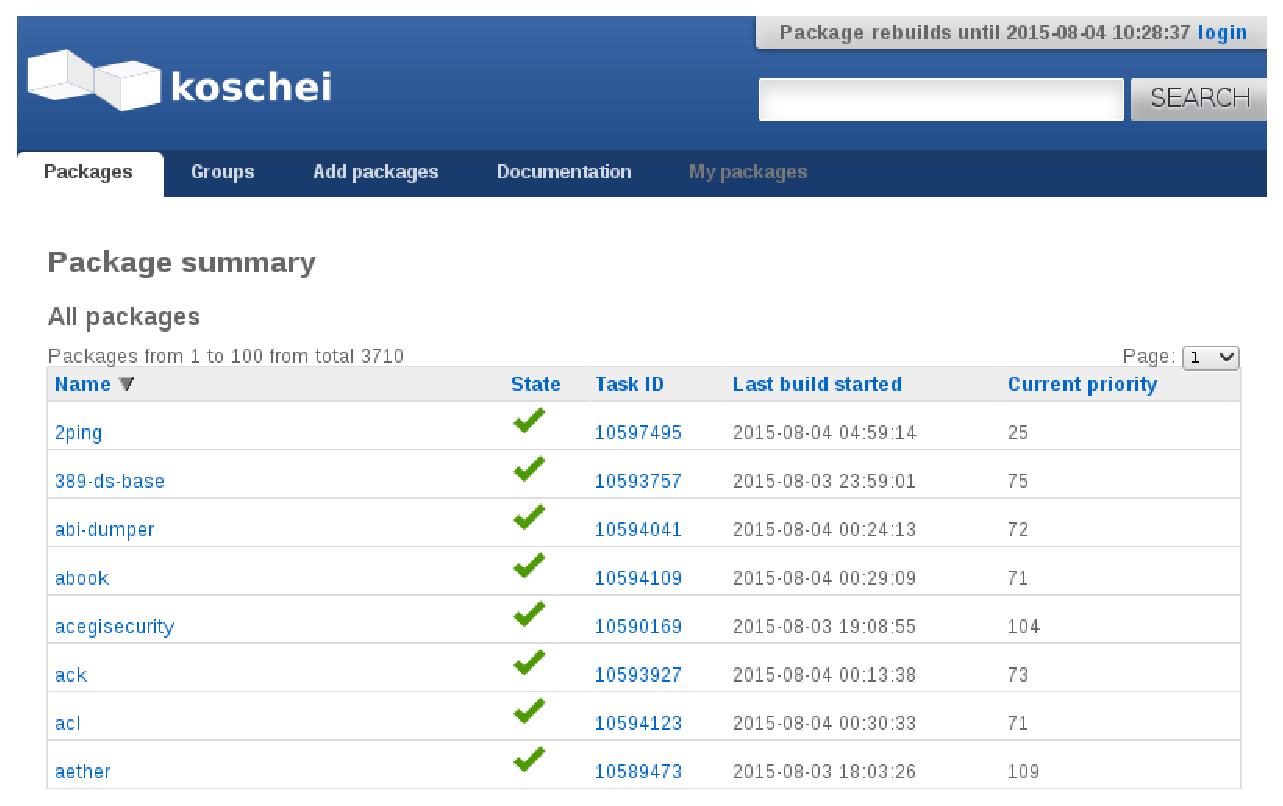
\includegraphics[scale=0.48]{koschei-frontend-1.eps}
  \end{center}
\end{frame}

\begin{frame}[fragile]
  \begin{center}
    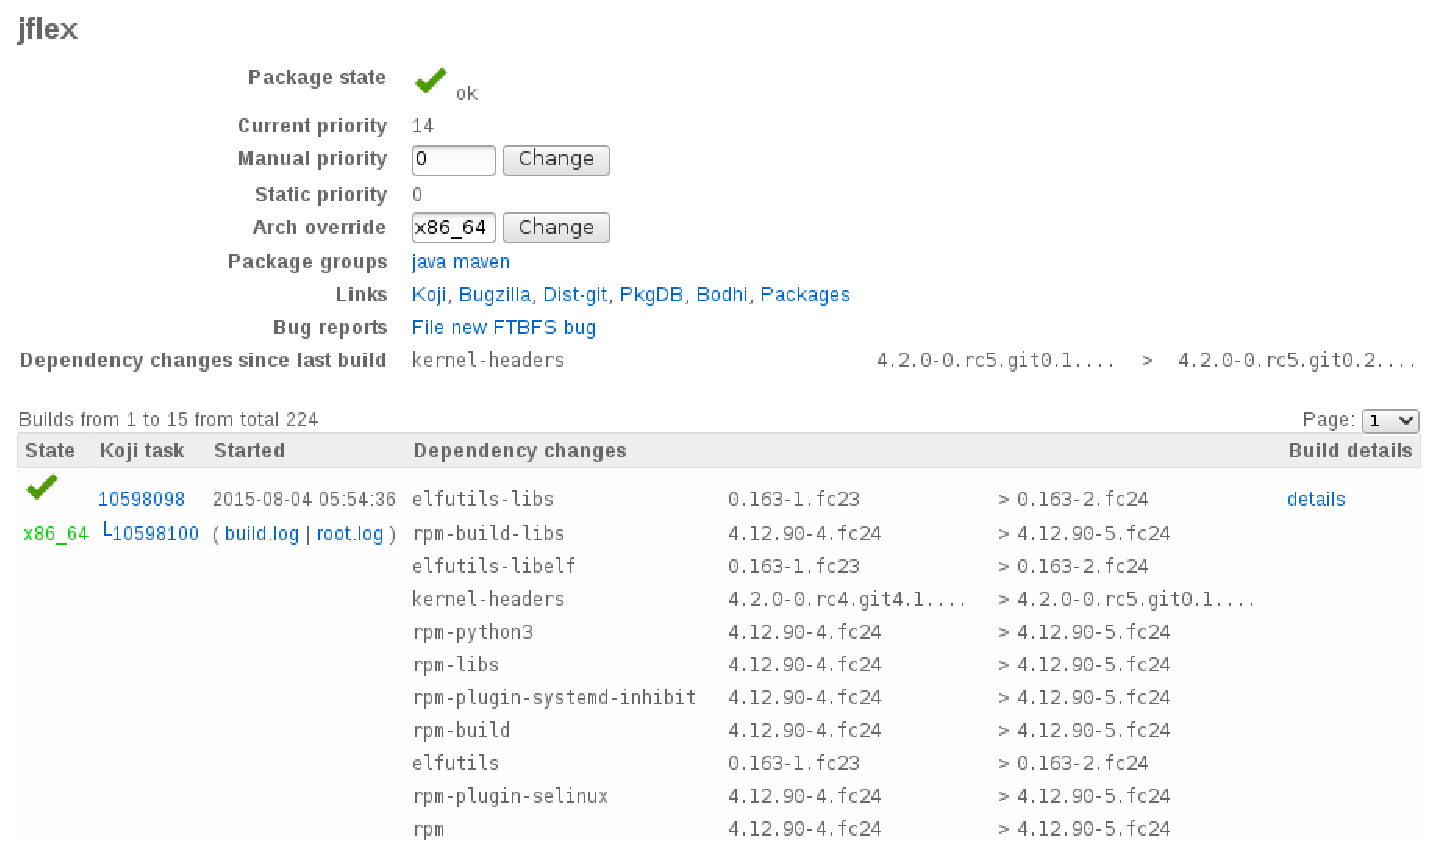
\includegraphics[scale=0.48]{koschei-frontend-2.eps}
  \end{center}
\end{frame}

\begin{frame}[fragile]
  \begin{center}
    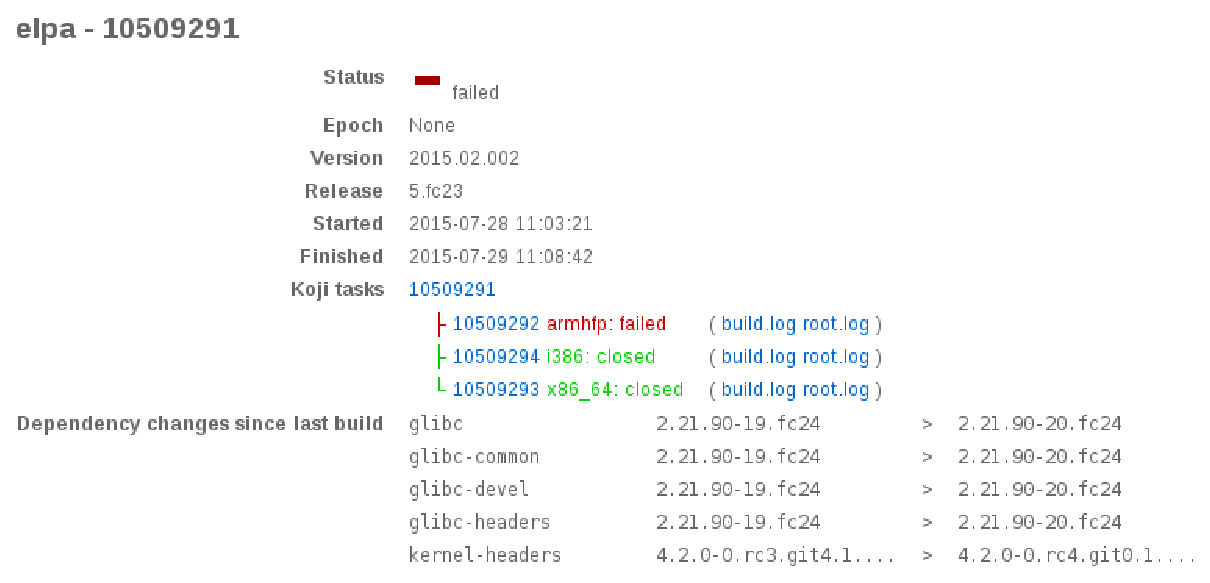
\includegraphics[scale=0.48]{koschei-frontend-3.eps}
  \end{center}
\end{frame}

\begin{frame}
  \frametitle{Current state}
  \begin{itemize}
    \item code at Github
    \item available in Fedora and EPEL 7
    \item running at Fedora infrastructure
    \item FMN filters
  \end{itemize}
\end{frame}

\begin{frame}
  \frametitle{Statistics}
  \begin{itemize}
    \item Monitored packages
    \begin{itemize}
% count of all packages:
%   select count(*) from package where ignored = false;
      \item 3715 packages
% count of all rawhide packages:
%   koji -q list-pkgs --tag f24 | wc -l
      \item 22 \% of all packages
% count of all packages in state OK:
%   select count(*) from package inner join build
%      on package.last_complete_build_id = build.id
%      where package.ignored = false and package.resolved = true and build.state = 3;
      \item 3644 OK (98.09 \%)
% count of all packages in state FAILING:
%   select count(*) from package inner join build
%      on package.last_complete_build_id = build.id
%      where package.ignored = false and package.resolved = true and build.state = 5;
      \item 58 failing (1.56 \%)
% count of all packages in state UNRESOLVED:
%   select count(*) from package where ignored = false and resolved = false;
      \item 13 unresolved (0.35 \%)
    \end{itemize}
    \item Scratch build rate
    \begin{itemize}
      \item 1 bulid every 36 s
      \item 100 builds/hour
      \item 2400 builds/day
      \item 876000 builds/year
    \end{itemize}
  \end{itemize}
\end{frame}


\section{Future}
\begin{frame}
  \frametitle{TODO}
  \begin{itemize}
    \item pkgdb2 integration
    \item UI improvements
    \item RPC / CLI interface
    \item immediate scratch build purging
    \item more fedmsg events
    \item non-rawhide tags?
    \item automatic bug filing?
  \end{itemize}
\end{frame}

\begin{frame}
  \frametitle{Links}
  \begin{itemize}
    \item Production instance
    \begin{itemize}
      \item \url{https://apps.fedoraproject.org/koschei}
    \end{itemize}
    \item Documentation
    \begin{itemize}
      \item \url{https://fedoraproject.org/wiki/Koschei}
    \end{itemize}
    \item Code repository
    \begin{itemize}
      \item \url{https://github.com/msimacek/koschei}
    \end{itemize}
  \end{itemize}
\end{frame}


% demo
%  - basic navigation
%  - groups
%  - sorting by state
%  - using links to build logs
%  - filling ftbfs bug (people may be afraid to click on it)
%  - reading the dependency changes
%  - adding fmn filter for ``my packages'' (or just showing how it looks like)


\mode<presentation> {
  \Rhbg{\frame{\theend}}
}

\end{document}
